\chapter{Dst指数}
\label{app:dst}
Dst指数のデータは地磁気世界資料センター京都(World Data Center for Geomagnetism, Kyoto)より調べた~\cite{wdc2022creditdst}。
Dst指数とは、地磁気擾乱の大きさを表す指数であり、地磁気擾乱が起きる際に発生する、地球を取り巻く環状の電流(Ring Current)がどの程度地球磁場をどのくらい打ち消すかを表したものである。
Dst指数は、4か所(Hermanus, Kakioka, Honolulu, San Juan)で観測された地磁気の南北成分をもとに1時間値で導出される~\cite{sugiura1986dst}。
実際に地磁気擾乱が発生した場合は、値が急激に減少し、大きな負の値を取る。
また、トロムソの解析結果との比較に用いたDst指数は暫定値(Provisional value)であり、昭和基地の解析結果との比較に用いたDst指数は速報値(Real-time value)である。
暫定値はノイズなどを人目で取り除いたデータから算出されているが、速報値はノイズ除去などの操作を行う前の生データから算出されているため正確ではない値を含んでいることに注意する必要がある~\cite{wdc2022aedst}。
本研究では、地磁気擾乱が起きたかの判断をするための目安として用いた。


\chapter{SOFIE}
\label{app:sofie}
SOFIE(Solar Occultation for Ice Experiment)は2007年3月から2023年3月まで、NASAのAIM(Aeronomy of Ice in the Mesosphere)衛星に搭載されて運用された~\cite{russell2009aeronomy,sofie2006sdl}。
AIM衛星は、極中間圏雲(PMC: Polar Mesospheric Cloud)の研究のために打ち上げられ、太陽同期軌道で周回する。
SOFIEでは、とくにPMCが形成される領域の大気における分子や温度、微粒子を観測するために設計され、5種類の分子(\ce{H2O}・\ce{CO2}・\ce{O3}・\ce{CH4}・\ce{NO})とPMCの消失を11の波長で観測し、流星により発生した粒子について3つの波長で観測している。
これらの観測からそれぞれの高度プロファイルデータが取得され、高度分解能はおよそ$2\ \mathrm{km}$である。
SOFIEは太陽掩蔽法を用いて、主に極域において観測が行われており、SOFIEに対して太陽が日の出や日の入りをする際に、地球大気の縁をかすめるように通過した太陽光について赤外分光観測を行う。
本研究においては、Version 1.3 Dataを用いており、\url{http://sofie.gats-inc.com/swdocs}より取得した。
トロムソのミリ波分子計による\ce{NO}の柱密度の導出を行った期間においては、トロムソ付近の緯度(およそ65 - 80\textdegree Nの範囲)で日の入りの観測を行っていたため、この観測データを用い、\ce{NO}の高度プロファイルデータを比較対象として用いた。


\chapter{POES/MetOp}
\label{app:poes}
POES/MetOp(Polar Orbiting Environmental Satellites/Meteorological Operational Satellites、以下POES衛星)はNOAA(アメリカ海洋大気庁: National Oceanic and Atmospheric Administration) Space Weather Prediction Centerによって開発・運用されており、太陽同期軌道で周回する衛星である~\cite{poes2013noaa}。
POES衛星にはSEM-2(Space Environment Monitor-2)という観測装置が搭載されており、TED(Total Energy Detector)とMEPED(Medium Energy Proton and Electron Detector)で構成される。
MEPEDは、高エネルギーイオンと高エネルギー電子のフラックスを測定しており、in situ観測で行われる。\par

高エネルギー電子の観測においては、4つのエネルギーバンドをもち($>40\ \mathrm{keV}$, $>130\ \mathrm{keV}$, $>287\ \mathrm{keV}$, $>612\ \mathrm{keV}$)、2つの角度(0\textdegree, 90\textdegree)のフラックスを測定する。
0\textdegree では天頂方向を向いて観測を行っており、90\textdegree では、0\textdegree に対して垂直であり、衛星の速度方向とは逆向きに設置されている~\cite{meped2013noaa}。\par

POES衛星は複数の衛星で構成されており、運用されいる衛星は時期によって異なる。
トロムソの\ce{NO}の柱密度の比較においては6基の衛星(METOP-01, METOP-02, METOP-03, NOAA-15, NOAA-18, NOAA-19)を用い、昭和基地の\ce{NO}の柱密度の比較においては5基の衛星(METOP-01, METOP-03, NOAA-15, NOAA-18, NOAA-19)を用いた。
POES衛星の観測データについては、\url{https://www.ngdc.noaa.gov/stp/satellite/poes/dataaccess.html}より取得した。\par

電子フラックスデータの選定においては、観測場所(トロムソ・昭和基地)付近に降り込んでくると予想されるものであるかどうかを観点において、以下の条件で行った。
\begin{enumerate}
    \item 0\textdegree の電子フラックスデータ
    \item L値
    \par
    L値(L-shellまたはL-value)とは、磁力線が磁気赤道を横切る際に、地球の中心からどの程度離れているかを地球の半径の何倍かで表したものである。
    本研究では、L値が$5.5-7.5$の範囲である電子フラックスデータを用いた

    \item MLT(Magnetic Local Time)とUT(Universal Time)
    \par
    MLTとは、一般に用いられる自転軸から定義されるLT(Local Time)とは異なり、地磁気極から定義されるものである。
    トロムソにおいてはMLTがUTに対して2.24時間進んでいて、昭和基地においてはUTと等しいと仮定した。
    これを踏まえて、条件にあうUTとMLTで観測された電子フラックスデータを用いた(図\ref{fig:app_poes_box})。
    図中の破線はMLTのUTに対する差の仮定に基づいて、$\mathrm{MLT}-\mathrm{UT}$軸のグラフに表したものである。
    この破線に沿って$\mathrm{MLT}\ 3h \times \mathrm{UT}\ 3h$のBoxを考える。
    このBox内に含まれる電子フラックスデータを用いる。
    \begin{figure}[htbp]
        \centering
        \begin{minipage}{.495\linewidth}
            \leftline{(a)}
            \centering
            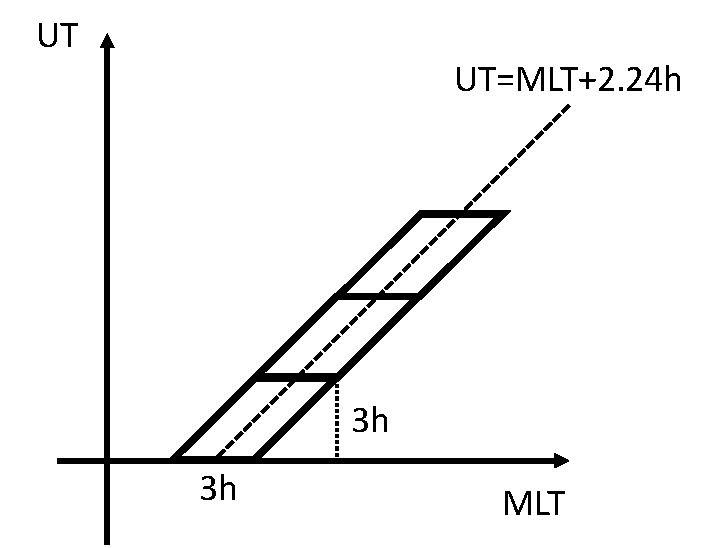
\includegraphics[scale=0.5]{master_thesis_contents/master_thesis_fig/app_poes_box_tromsoe.pdf}
        \end{minipage}
        \begin{minipage}{.495\linewidth}
            \leftline{(b)}
            \centering
            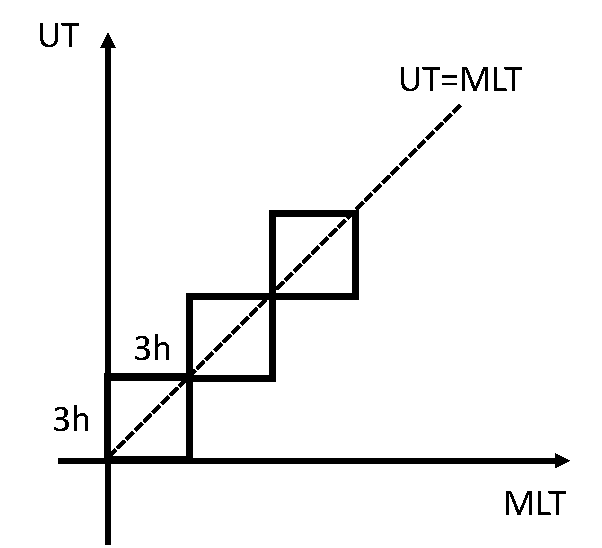
\includegraphics[scale=0.5]{master_thesis_contents/master_thesis_fig/app_poes_box_syowa.pdf}
        \end{minipage}
        \caption{電子フラックスデータの3時間平均の値の計算に用いるBox (a) トロムソの場合 (b) 昭和基地の場合}
        \label{fig:app_poes_box}
    \end{figure}
\end{enumerate} \par
以上の条件を満たした電子フラックスデータについて、図\ref{fig:app_poes_box}で示したBoxごとに平均値を計算し3時間平均値としてプロットを行った。


\chapter{OMNI Data Set}
\label{app:omni}
OMNI Data SetはNASAから提供されており、主に磁気圏と電離層における太陽風の影響の調査をサポートすることを目的としたものである~\cite{king2005solar,king2023omni}。
本研究では、OMNI Data Setの中でもHigh Resolution OMNI data set(HRO)を用いた。
HROは1分と5分の時間分解能のデータにより構成されており、はじめは3つの衛星(ACE・Wind・IMP 8)のデータによって構成され($2005-2006$年)、後の2007年にGeotail、2009年にGOESのプロトンのフラックスデータが追加された。
\par
OMNI Data Setの中でも本研究で用いたデータは以下の5つである。
\begin{enumerate}
    \item 地球磁場の南北$z$成分$B_z$(GSM)$[\mathrm{nT}]$
    \par
    地球磁場の南北成分を表す。
    GSM(Geocentric Solar Magnetospheric system)とは、座標系の一つである~\cite{russell1971geophysical}。
    地球から太陽までを$x$軸とし、$y$軸は地球の磁気双極子に対して垂直であり、$z$軸は$y-z$平面が双極子軸を含むように定義される。
    なお、$z$軸は北極の磁極の方向を正とする。

    \item 太陽風の速さ$[\mathrm{m/s}]$
    % 太陽風の速さ
    \item プロトン密度$[\mathrm{n/cc}]$
    % プロトン密度
    \item AE指数$[\mathrm{nT}]$
    \par
    AE指数はサブストームに伴う電流の大きさを表すものであり、高緯度オーロラ帯の12か所磁場変動の最大値と最小値の差をとったものである。
    AE指数においてはトロムソの\ce{NO}の柱密度の比較においてのみ用いている。
    昭和基地の解析した期間についてはAE指数は\today 時点で公開されていないため、昭和基地における柱密度との比較ではAE指数は用いていない。

    \item SYM/H$[\ \mathrm{nT}]$
    \par
    SYM/HはDst指数の1分値に相当するものである~\cite{wdc2009asysym}。

\end{enumerate}


\chapter{発表実績}
\begin{itemize}
    \item H Goto, A Mizuno, T Nagahama, T Nakajima, S Nozawa, Y Kojima, T Kawabata, R Fujimori, K Suzuki and Y Ogawa. Research on the Analysis of Nitric Oxide Molecular Spectral Data with Millimeter-Wave Spectroscopic Observations in Troms\o , Norway. JpGU(Japan Geoscience Union Meeting), Online, Jun. 2021.
    \item H Goto, T Nakajima, T Nagahama, S Nozawa, Y Kojima, T Kawabata, R Fujimori, K Suzuki, Y Ogawa, A Mizuno. A study on the relationship between NO column density and high-energy electrons based on the mm-wave observation at Troms\o . SGEPSS(Society of Geomagnetism and Earth, Planetary and Space Sciences), Online, Nov. 2021.
    \item H Goto, A Mizuno, T Nakajima, T Nagahama. A study on the relationship between NO column density and high-energy electrons based on the mm-wave observation at Syowa station. SGEPSS(Society of Geomagnetism and Earth, Planetary and Space Sciences), 東北大学青葉山北キャンパス, Sep. 2023.
\end{itemize}
